\section{N-Task Extension}

In this section we extend our formulation to task chains of arbitrary length and with forks and merges. We do this through the use of our 2-task and 3-task formulation insights, as constraints in an optimization problem which can then be solved using constrained optimization software.

We again formulate any end-to-end deadlines as the combination of several local constraints. In particular, there is a local freshness constraint from each producer task $i$ to its consumer task $j$. Let each pair $\{i,j\} \in E$ and $E_k$ be the subset of pairs in a chain for a particular freshness constraint $D_k$. Each of these local freshness constraints are between two tasks, and thus we can ensure the consuming task receives data according to the local constraint by using Lemma~\ref{lem:2TaskResult}: $P_i \leq \frac{d_{i \to j} + E^{l,min}_i}{2}$, with this inequality being equal in order to minimize utilization.

As we saw in the three task scenario, it is sufficient to solve for these local deadlines as they can be transformed into periods for each task. Our optimization follows suit by using this idea in the constraints and then solving for the local deadlines which yield the least utilization. Once a solution is found we convert the local constraints into periods for producer tasks. Hence, although the optimization problems will describe solving for local constraints they do not differ from the general problem statement presented earlier. A concrete example to illustrate how we will encode our freshness constraints, and hence period selection, is shown in Figure ~\ref{fig:fork-merge}.

\begin{figure}[!ht]
	\centering
	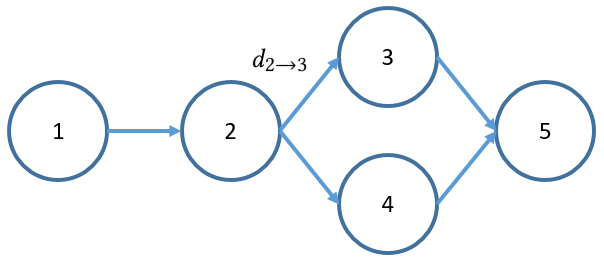
\includegraphics[width=0.3\textwidth]{figures/fork-merge}
	\caption{Example of chain with fork and merge.}
	\label{fig:fork-merge}
\end{figure}

Suppose data consumed by task $2$ must be at most 10 time units old and data consumed by task $5$ must be at most 50 time units old. Our optimization would look like the following:

\begin{align*}
	\text{Given: }& E^{*,*}_i \text{ for each } i \text{ in } 1 \ldots 5\\
	\text{Find: }& P_1, \ldots, P_5\\
	\text{(i.e., Find: }& d_{1 \to 2}, d_{2 \to 3}, d_{2 \to 4}, d_{3 \to 5}, \text{ and } d_{4 \to 5}\text{)}\\
	\text{Minimize: }& \text{Maximum Utilization} \\
	\text{Subject To: }& d_{1 \to 2} \le 10 \\
	\text{ and: }& d_{1 \to 2} + E^{u,max}_2 + d_{2 \to 3} + E^{u,max}_3 + d_{3 \to 5} \le 50 \\
	\text{ and: }& d_{1 \to 2} + E^{u,max}_2 + d_{2 \to 4} + E^{u,max}_4 + d_{4 \to 5} \le 50 \\
	\text{ and: }& \text{each } d_{\star \to \star} > 0
\end{align*}

\noindent From here on out $\star$ is used as a wild card for any valid value that can be used in its place.

Note that this can be easily applied to several pieces of data and is not limited to a single datum. Constraints can be added for several pieces of data and the solution will select the most stringent period required for any one particular data piece.

Below we present the optimization problem for any chain and deadlines. Since we do not know the periods of the tasks during the optimization, we must represent utilization using the provided parameters. We do this using the local deadlines. The optimization problem is as follows:

\begin{align*}
	\text{Given: }& E^{l,min}_i, E^{u,max}_i \text{ for each } i \text{ in } 1 \ldots n\\
	\text{Find: }& d_{i \to j} \text{ for each } \{i,j\} \in E\\
	\text{Minimize: }& U = \sum_{i : \{i,\star\} \in E} \frac{E^{u,max}_i}{P_i} = \sum_{i : \{i,\star\} \in E} \frac{2 \times E^{u,max}_i}{\min(d_{i \to \star}) + E^{l,min}_i} \\
	\text{Subject To: }& \forall k, \sum_{i : \{i,\star\} \in E_k} E^{u,max}_i + \sum_{i : \{i,j\} \in E_k} d_{i \to j} \le D_k \\
	\text{ and: }& \forall{\{i,j\} \in E}, d_{i \to j} > 0
\end{align*}

Note the problem is not linear due to the utilization objective, but the utilization does monotonically increase as any one local deadline decreases within the constraints. As each variable changes the objective in the same manner (no saddles) and the constraints are are simple addition and comparisons, this problem appears to be convex. While we cannot provide an analytical solution for the $n$ task case with this problem, it performs the same optimization as the analytical case would for any $n$.

Given our intuition from the theory evaluation (later) which suggests earlier chain tasks are often assigned higher priority, we extended the optimization problem to be specific to rate-monotonic scheduling by adding additional constraints dictating that the period of each producing task in a chain is less than or equal to the period of its consuming task. Note that this does not always hold in the 3 task scenario depending upon the parameters, but it is a trend we noticed and was a basis for our intuition. The added constraints will cause earlier tasks to have higher priority with the intention of pushing new values through the chain before consuming older ones. The RM-specific formulation is the same as above but with the added constraint:
\begin{align*}
	&\forall{\{i,j\} \in E}, P_{i} \le P_{j} \\
	\implies &\forall{\{i,j\} \in E}, \forall k : \{j,k\} \in E, \frac{d_{i \to j} + E^{l,min}_i}{2} \le \frac{d_{j \to k} + E^{l,min}_{j}}{2}\\
	%\implies &\forall{\{i,j\} \in E}, \forall k : \{j,k\} \in E, d_{i \to j} + E^{l,min}_i \le d_{j \to k} + E^{l,min}_{j}\\
\end{align*}

Other constraints may be added by the designer if desired. For example, in either formulation, if a polling task $T_1$ must run at least every 50 time units as per the Nyquist requirement, an additional constraint could be added: $P_1 \le 50$. Note $P_1$ would have to converted to use the local deadline notation similar to above.

Finally, note that this method works for multiple disconnected task chains. That is, the requirements of each chain can be encoded in the optimization constraints while the objective function remains the utilization of all tasks. An entire system of complex task chains with forks, merges, and multiple data pieces can be simultaneously optimized in a single optimization problem.